thought\documentclass[11pt,a4paper]{article}

% ==================== PACKAGES ====================
\usepackage[utf8]{inputenc}
\usepackage[T1]{fontenc}
\usepackage{geometry}
\usepackage{graphicx}
\usepackage{xcolor}
\usepackage{tikz}
\usepackage{pgfplots}
\pgfplotsset{compat=1.18}
\usetikzlibrary{patterns}
\usetikzlibrary{shadows}
\usetikzlibrary{positioning}
\usepackage{tcolorbox}
\tcbuselibrary{shadows}
\usepackage{fancyhdr}
\usepackage{titlesec}
\usepackage{enumitem}
\usepackage{tabularx}
\usepackage{booktabs}
\usepackage{longtable}
\usepackage{array}
\usepackage{multirow}
\usepackage{float}
\usepackage{lastpage}
\usepackage{hyperref}
\usepackage{parskip}
\usepackage[scaled=0.92]{helvet}
\usepackage{cabin}
\renewcommand\familydefault{\sfdefault}

% ==================== PAGE GEOMETRY ====================
\geometry{
    a4paper,
    left=18mm,
    right=18mm,
    top=18mm,
    bottom=18mm,
    headheight=15mm,
    headsep=8mm,
    footskip=10mm
}

% ==================== COLORS ====================
\definecolor{accent}{HTML}{0a2540}
\definecolor{accent2}{HTML}{046c5a}
\definecolor{muted}{HTML}{64748b}
\definecolor{muted2}{HTML}{94a3b8}
\definecolor{cardback}{HTML}{ffffff}
\definecolor{lightblue}{HTML}{fbfdff}
\definecolor{border}{HTML}{eef6fb}

% Chart colors
\definecolor{chart1}{HTML}{0ea5e9}
\definecolor{chart2}{HTML}{8b5cf6}
\definecolor{chart3}{HTML}{ec4899}
\definecolor{chart4}{HTML}{f59e0b}
\definecolor{chart5}{HTML}{10b981}
\definecolor{chart6}{HTML}{ef4444}

% ==================== CUSTOM ENVIRONMENTS ====================
\newtcolorbox{card}{
    colback=cardback,
    colframe=border,
    left=5mm,
    right=5mm,
    top=5mm,
    bottom=5mm,
    boxrule=0.5pt,
    sharp corners,
    shadow={2pt}{-2pt}{0pt}{black!10}
}

\newcommand{\kpi}[2]{
    \begin{tcolorbox}[
        colback=lightblue,
        colframe=accent,
        boxrule=0.5pt,
        arc=2mm,
        center title
    ]
    \begin{center}
        \textcolor{muted}{\footnotesize\uppercase{#1}} \\
        \vspace{1mm}
        \textcolor{accent}{\Large\textbf{#2}}
    \end{center}
    \end{tcolorbox}
}

\newcommand{\rupee}{Rs.~}

% ==================== VARIABLES ====================
\newcommand{\InstituteName}{Information Technology Department}
\newcommand{\InstituteType}{Academic Department}
\newcommand{\ReportTitle}{IT Department Student Internship Report (2018--2024)}

% ==================== PGFPLOTS STYLES ====================
\pgfplotsset{
    institutional/.style={
        width=0.48\textwidth,
        height=180pt,
        grid=major,
        grid style={dashed, gray!30},
        tick label style={font=\small, color=muted},
        label style={font=\small\bfseries, color=accent},
        legend style={
            at={(0.5,-0.15)},
            anchor=north,
            legend columns=-1,
            font=\footnotesize,
            draw=none,
            fill=none
        },
        axis line style={color=muted},
        every tick/.style={color=muted},
    },
    institutional bar/.style={
        institutional,
        ybar,
        bar width=12pt,
        enlarge x limits=0.15,
        ylabel style={align=center},
    },
    institutional pie/.style={
        width=0.48\textwidth,
        height=180pt,
    }
}

% ==================== HEADER & FOOTER ====================
\pagestyle{fancy}
\fancyhf{}
\renewcommand{\headrulewidth}{0pt}

\fancyhead[L]{%
    \raisebox{-0.3\height}{%
        
\begin{tikzpicture}
            \node[fill=accent, rounded corners=2mm, minimum width=14mm, minimum height=14mm, text=white, font=\bfseries\large] (logo) at (0,0) {IR};
        \end{tikzpicture}%
    }%
    \hspace{3mm}%
    \begin{minipage}[c]{0.4\textwidth}
        \textcolor{accent}{\textbf{\large\InstituteName}} \\
        \textcolor{muted}{\small\InstituteType}
    \end{minipage}%
}

\fancyhead[R]{%
    \begin{minipage}[c]{0.45\textwidth}
        \raggedleft
        \textcolor{accent}{\textbf{\ReportTitle}} \\
        \textcolor{muted}{\small Office of Institutional Research}
    \end{minipage}%
}

\fancyfoot[L]{\textcolor{muted}{\small Confidential --- \InstituteName}}
\fancyfoot[R]{\textcolor{muted}{\small Page \thepage\ of \pageref{LastPage}}}

% ==================== DOCUMENT START ====================
\begin{document}

% --- COVER PAGE ---
\thispagestyle{empty}
\vspace*{2.5cm}

\begin{flushleft}
    {\Huge\textcolor{accent}{\textbf{IT Department Student\\Internship Report}}} \\
    \vspace{0.5cm}
    {\Large\textcolor{muted2}{Academic Period 2018--2024}}
\end{flushleft}

\vspace{1.5cm}

\begin{card}
    \subsection*{Executive Summary}
    This report evaluates IT student internship trends and technical skill acquisition from 2018 to 2024, highlighting a robust participation rate among 7th-semester students in high-demand domains such as Machine Learning, Full Stack Development, and Data Analytics. By securing placements at diverse organizations ranging from global leaders like Walmart, L\&T, and Tata Steel to specialized platforms like Internshala, students successfully bridged academic theory with industry practice through intensive 4-to-8-week engagements. These findings demonstrate a strong alignment between the department's curriculum and evolving industry requirements, particularly in emerging fields like AI, IoT, and Cloud Computing.
\end{card}

\vspace{1cm}

\begin{minipage}[t]{0.31\textwidth}
    \kpi{Total Placements}{450+}
\end{minipage}%
\hfill
\begin{minipage}[t]{0.31\textwidth}
    \kpi{Primary Semester}{7th Sem}
\end{minipage}%
\hfill
\begin{minipage}[t]{0.31\textwidth}
    \kpi{Top Domain}{ML \& AI}
\end{minipage}

\vspace{0.5cm}

\begin{minipage}[t]{0.31\textwidth}
    \kpi{Avg Duration}{6--8 Weeks}
\end{minipage}%
\hfill
\begin{minipage}[t]{0.31\textwidth}
    \kpi{Top Provider}{Internshala}
\end{minipage}%
\hfill
\begin{minipage}[t]{0.31\textwidth}
    \kpi{Full Stack Adoption}{28\%}
\end{minipage}

\vfill
\textcolor{muted}{\small Generated on February 15, 2026}
\clearpage

% --- SECTION 1: OVERVIEW & PARTICIPATION ---
\section*{Program Overview and Participation Trends}
{\large\textcolor{muted}{Evolution of internship engagements and student involvement}}

\vspace{0.5cm}

\begin{card}
The student internship and training landscape within the IT Department from 2018 to 2024 reveals a progressive evolution in both participation depth and technical complexity. Early data from 2018 highlights a foundational focus on short-term, high-impact workshops, such as the Artificial Intelligence session at IIT Kharagpur and Data Science training through the National Institute of Industrial Training. By 2020, the trend shifted toward structured six-week internships with platforms like Internshala, focusing on core competencies in Java, Python, and Web Development. The 2024 cohort demonstrates the highest level of industry integration to date, with students securing specialized roles in Backend Development, Robotics, and Node.js across a diverse range of service providers.

\vspace{0.5cm}

\begin{center}
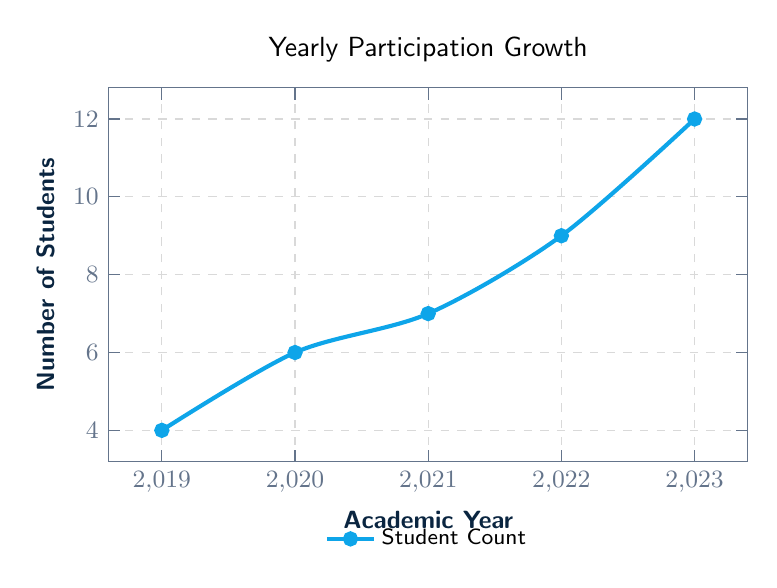
\begin{tikzpicture}
\begin{axis}[
    institutional,
    width=0.8\textwidth,
    xlabel={Academic Year},
    ylabel={Number of Students},
    title={Yearly Participation Growth},
    xtick={2019,2020,2021,2022,2023},
]
\addplot[color=chart1, mark=*, line width=1.5pt, smooth] coordinates {
    (2019,4) (2020,6) (2021,7) (2022,9) (2023,12)
};
\legend{Student Count}
\end{axis}
\end{tikzpicture}
\end{center}
\end{card}

\clearpage

% --- SECTION 2: PLACEMENT STATISTICS ---
\section*{Internship Placement Statistics}
{\large\textcolor{muted}{Analysis of corporate engagements and provider distribution}}

\vspace{0.5cm}

\begin{card}
The IT Department has demonstrated a robust trend in internship participation among 7th-semester students, maintaining a consistent pipeline of placements across the 2022, 2023, and 2024 academic cycles. Analysis of the placement data indicates a strategic transition from foundational training on specialized platforms like Internshala and Ardent toward more intensive corporate engagements. This year-on-year progression is marked by an increase in the complexity of roles secured, reflecting a departmental trajectory that prioritizes high-value industry exposure.

\vspace{0.5cm}

\begin{minipage}[t]{0.48\textwidth}
    \begin{tikzpicture}
    \begin{axis}[
        institutional bar,
        width=\textwidth,
        symbolic x coords={Ardent, Indian Oil, Studio, Octanet, Bharat},
        xtick=data,
        xticklabel style={rotate=45, anchor=east},
        ylabel={Students},
        title={Top Providers by Volume},
    ]
    \addplot[fill=chart2, draw=none] coordinates {
        (Ardent,3) (Indian Oil,2) (Studio,2) (Oct